\documentclass{ctexart}
\usepackage{ctex}
\usepackage{fontspec}
\usepackage{xcolor}
\usepackage{graphicx}
\usepackage{listings}
\lstset{
	language = Java,
	backgroundcolor = \color{yellow!10},    % 背景色:淡黄
	basicstyle = \tiny\ttfamily,           % 基本样式 + 小号字体
	rulesepcolor= \color{gray},             % 代码块边框颜色
	breaklines = true,                  % 代码过长则换行
	numbers = left,                     % 行号在左侧显示
	numberstyle = \small,               % 行号字体
	keywordstyle = \color{blue},            % 关键字颜色
	commentstyle =\color{gray},        % 注释颜色
	stringstyle = \color{red!100},          % 字符串颜色
	frame = shadowbox,                  % 用(带影子效果)方框框住代码块
	showspaces = false,                 % 不显示空格
	columns = fixed,                    % 字间距固定
	%escapeinside={<@}{@>}              % 特殊自定分隔符:<@可以自己加颜色@>
	morekeywords = {as}               % 自加新的关键字(必须前后都是空格)      % 删除内定关键字;删除错误标记的关键字用deletekeywords删!
}
\title{\heiti \zihao{2} 简单的画图}
\date{\today}
\author{孙博言 \and 2011756 \and 计算机学院}
\begin{document}
\maketitle
\section{功能展示}
\begin{figure}[htbp]
    \centering
    \caption{界面展示}
    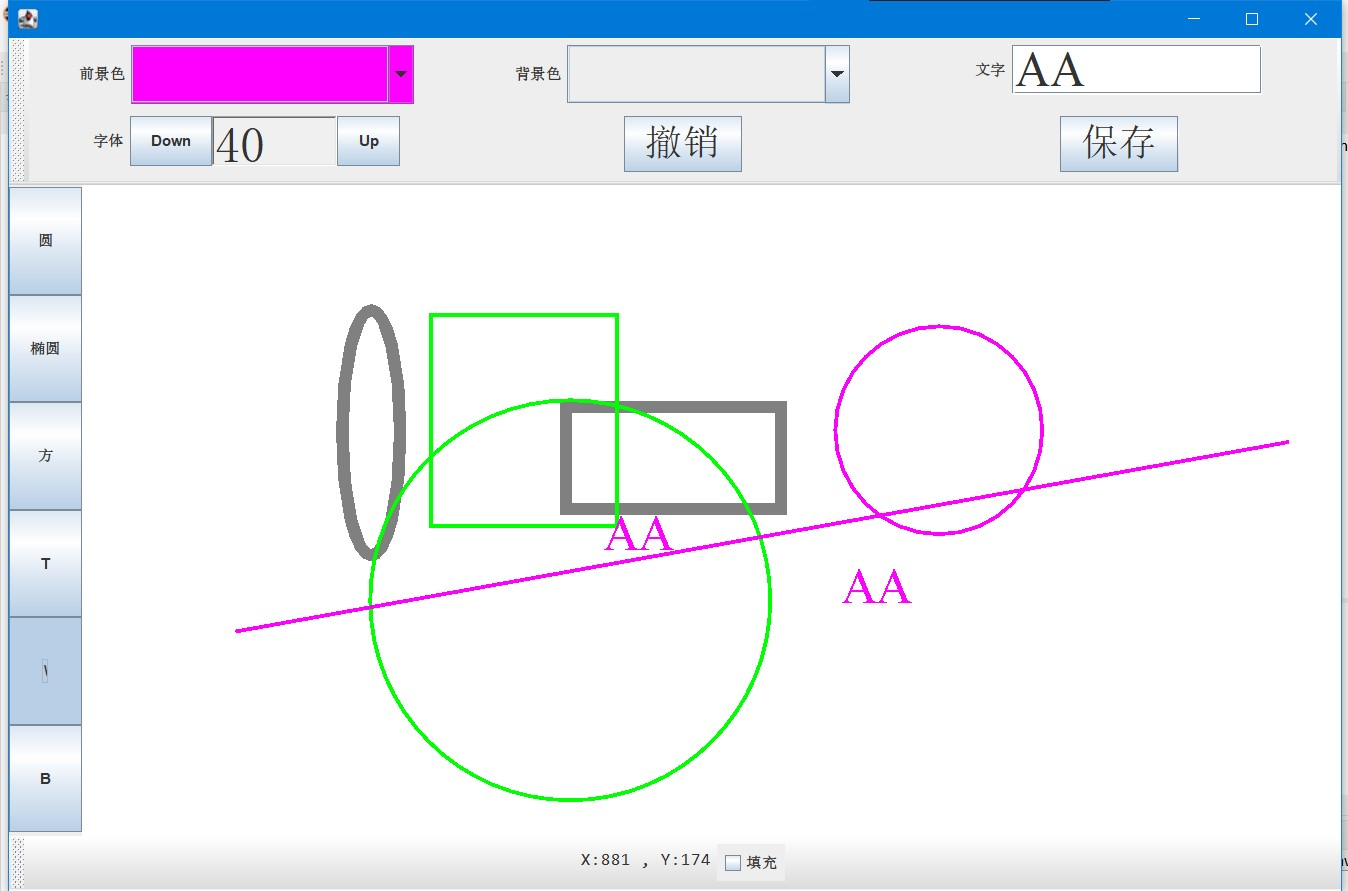
\includegraphics[scale = 0.4]{2.jpg}
    \label{fig:1}
\end{figure}
\begin{figure}[htbp]
    \centering
    \caption{形状总览}
    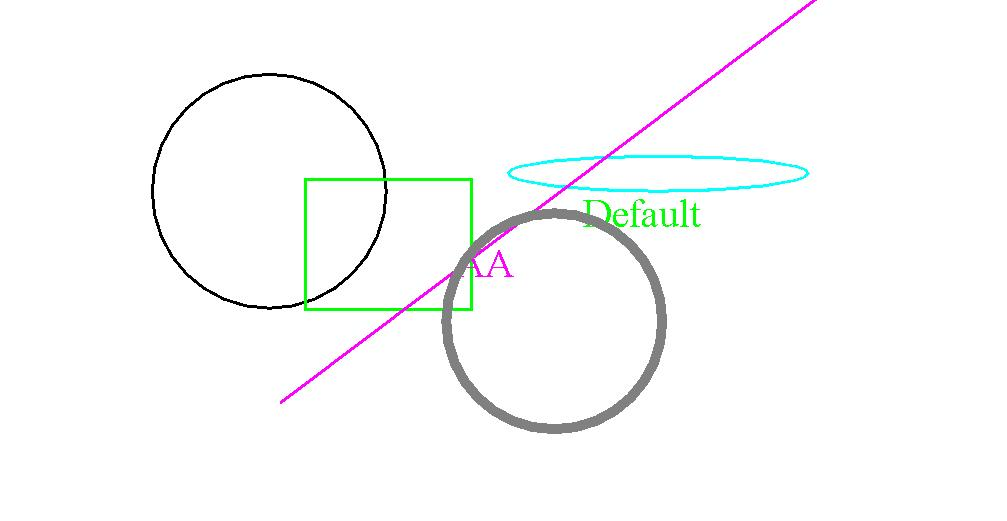
\includegraphics[scale = 0.4]{1.jpg}
    \label{fig:2}
\end{figure}
\begin{figure}[htbp]
    \centering
    \caption{线条加粗}
    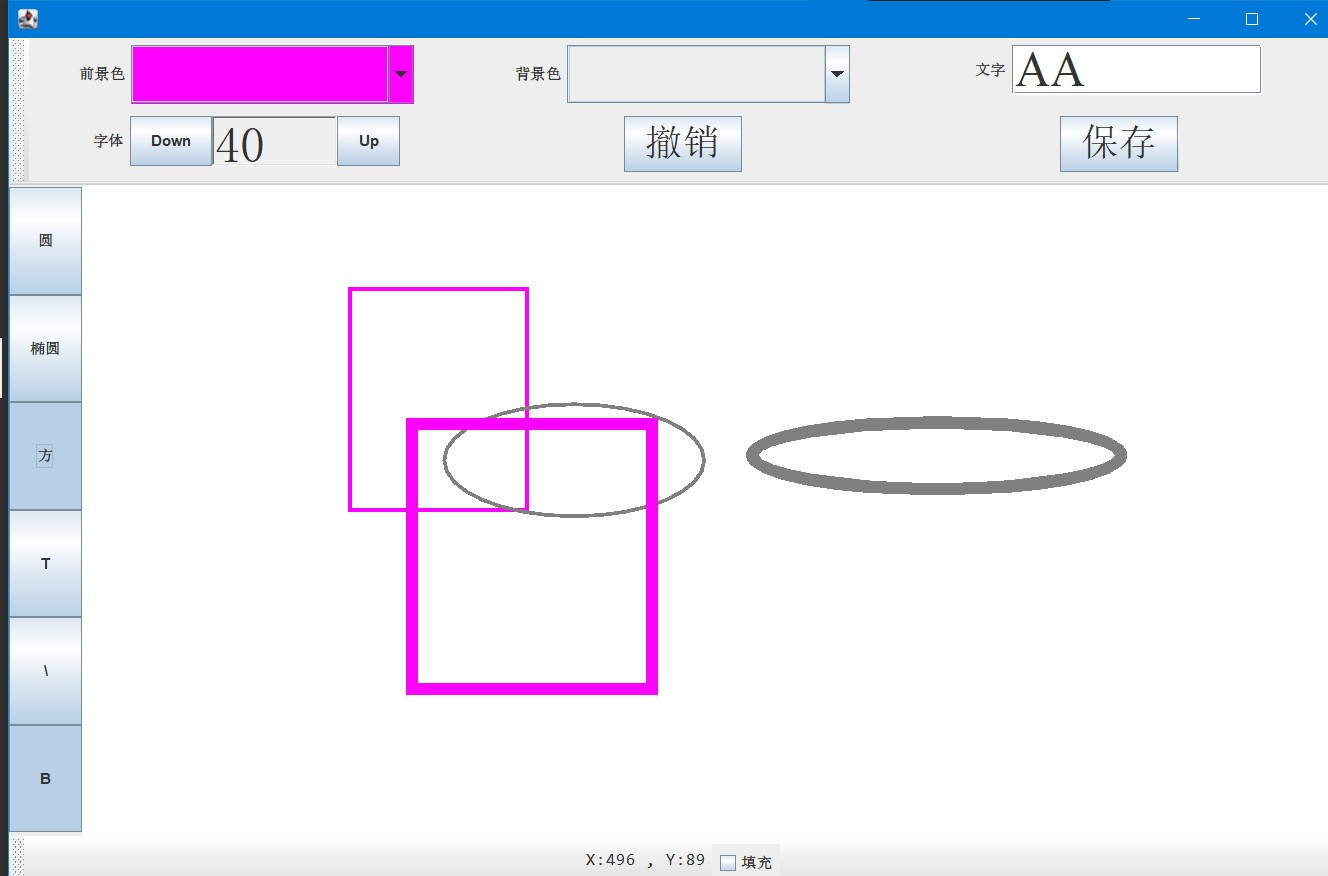
\includegraphics[scale = 0.4]{3.jpg}
    \label{fig:3}
\end{figure}
\begin{figure}[htbp]
    \centering
    \caption{局部填充}
    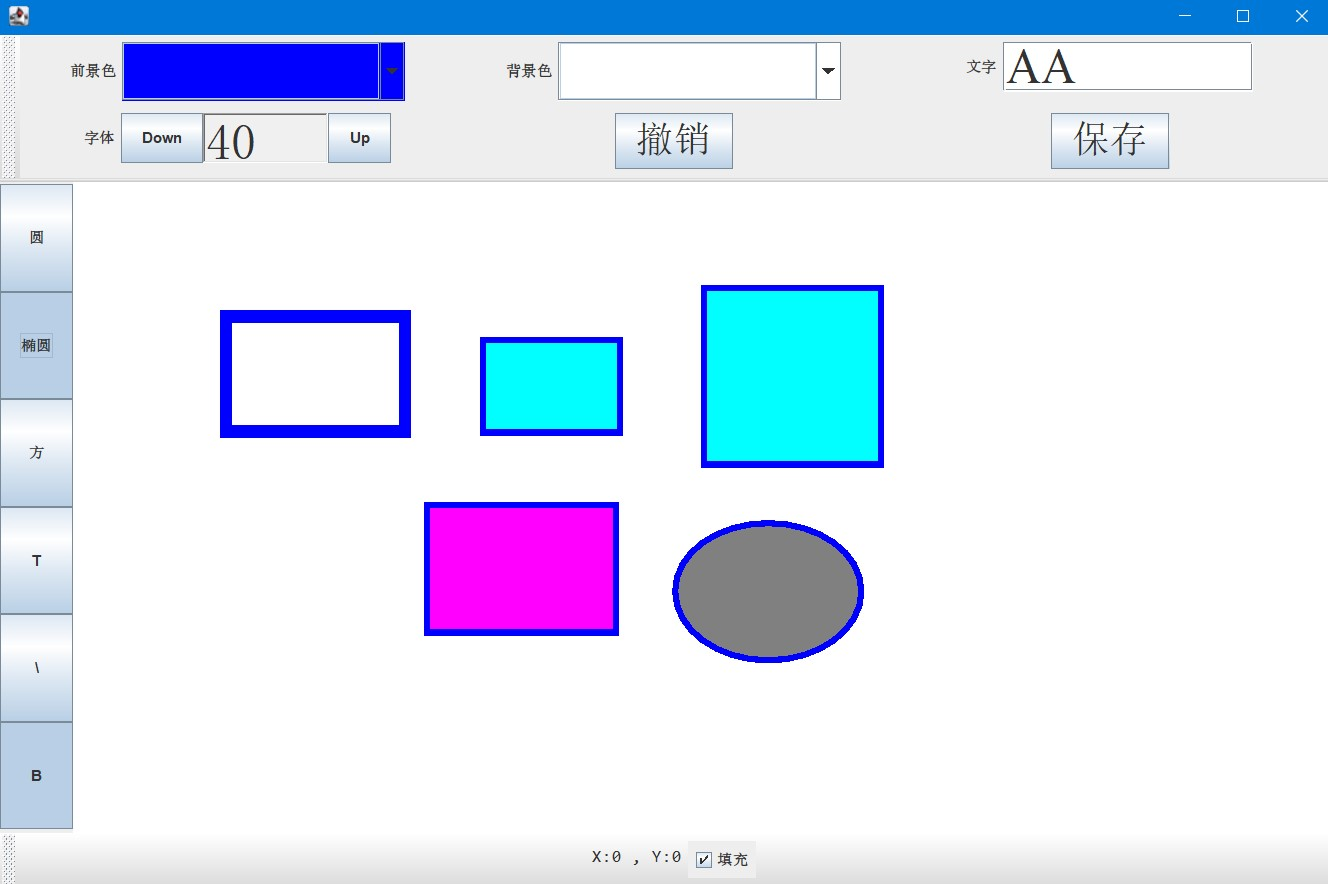
\includegraphics[scale = 0.4]{4.jpg}
    \label{fig:4}
\end{figure}
\begin{figure}[htbp]
    \centering
    \caption{字体大小}
    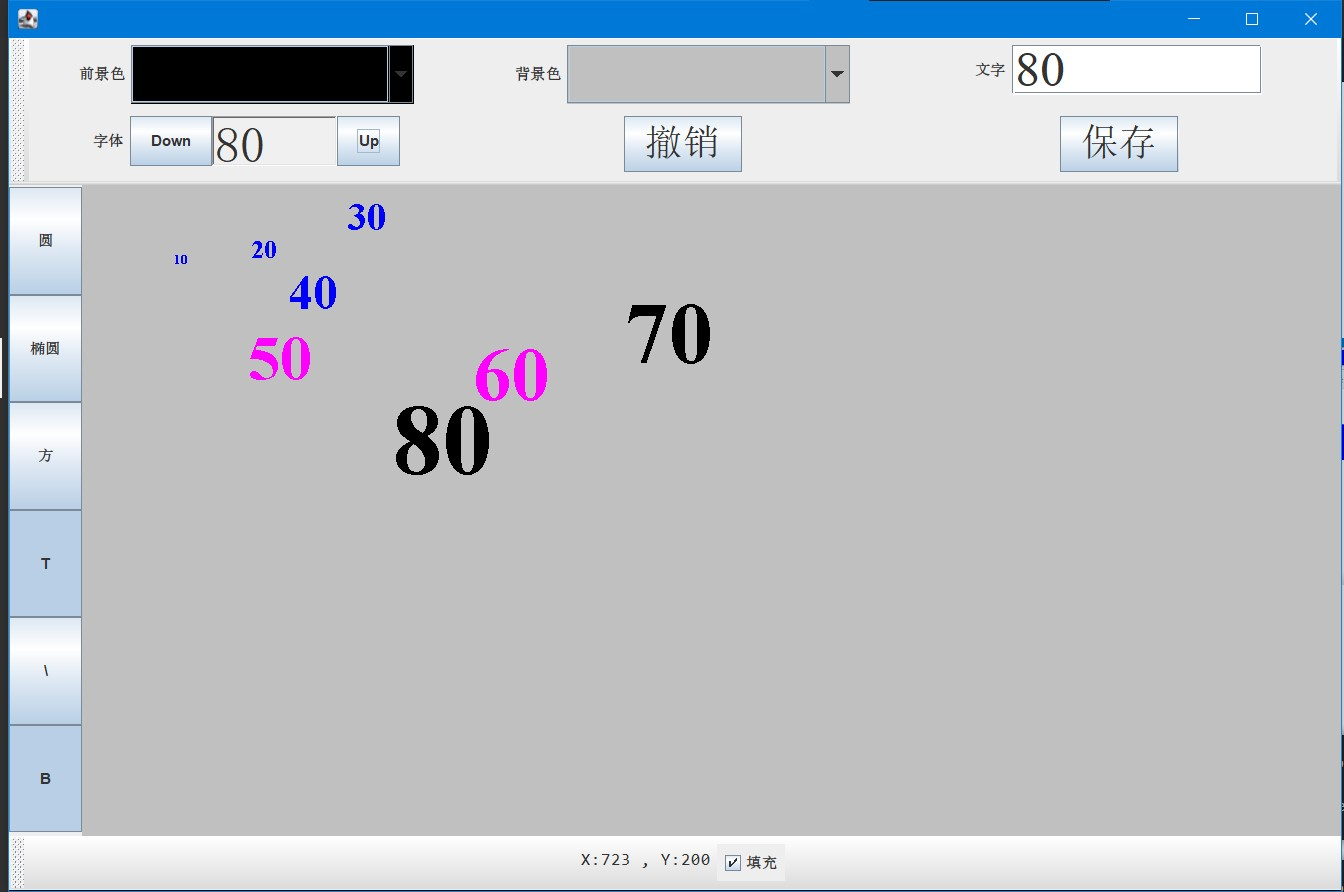
\includegraphics[scale = 0.4]{5.jpg}
    \label{fig:5}
\end{figure}
\begin{figure}[htbp]
    \centering
    \caption{自动缓存图片(形状数目每超过10)}
    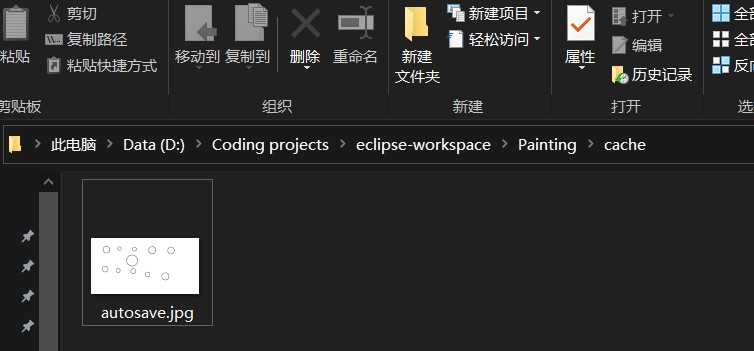
\includegraphics[scale = 0.7]{6.jpg}
    \label{fig:6}
\end{figure}

\begin{figure}[htbp]
    \centering
    \caption{自动缓存图片(形状数目每超过10)}
    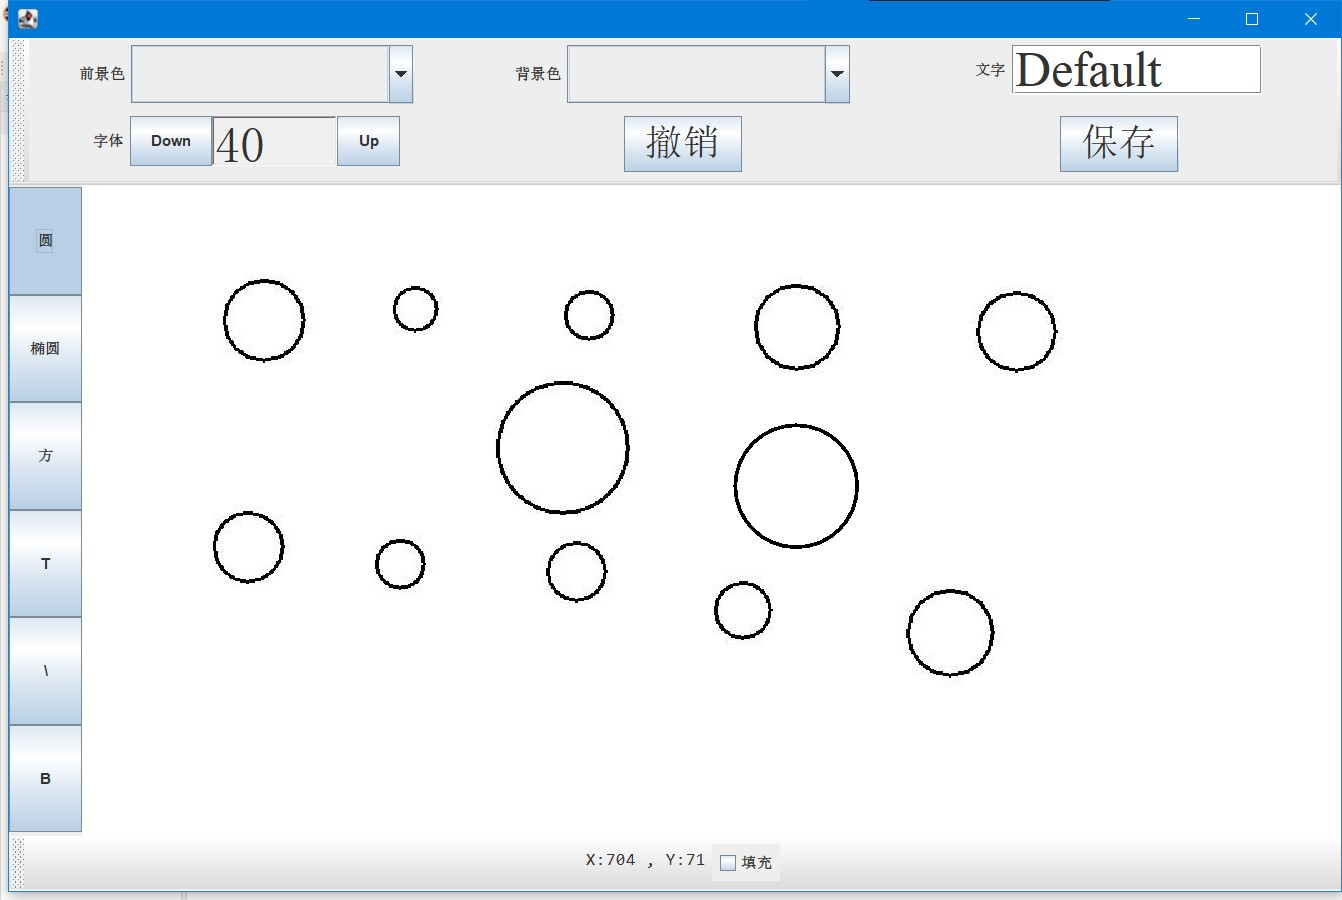
\includegraphics[scale = 0.4]{7.jpg}
    \label{fig:7}
\end{figure}
\begin{figure}[htbp]
    \centering
    \caption{在10步以内的动作可以撤回(可自行运行代码尝试)}
    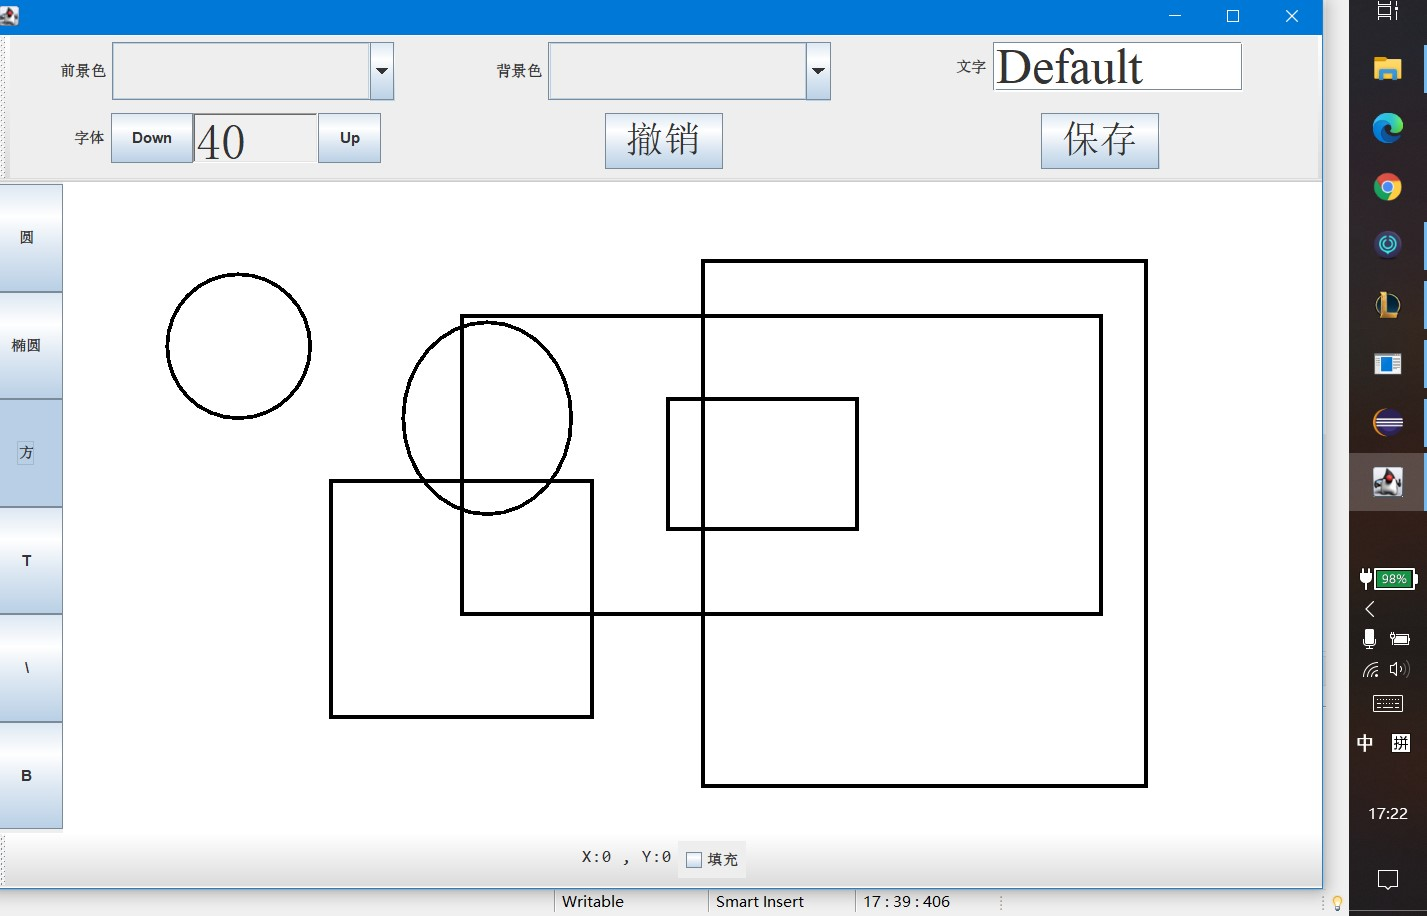
\includegraphics[scale = 0.4]{8.jpg}
    \label{fig:8}
\end{figure}
\begin{figure}[htbp]
    \centering
    \caption{撤回后}
    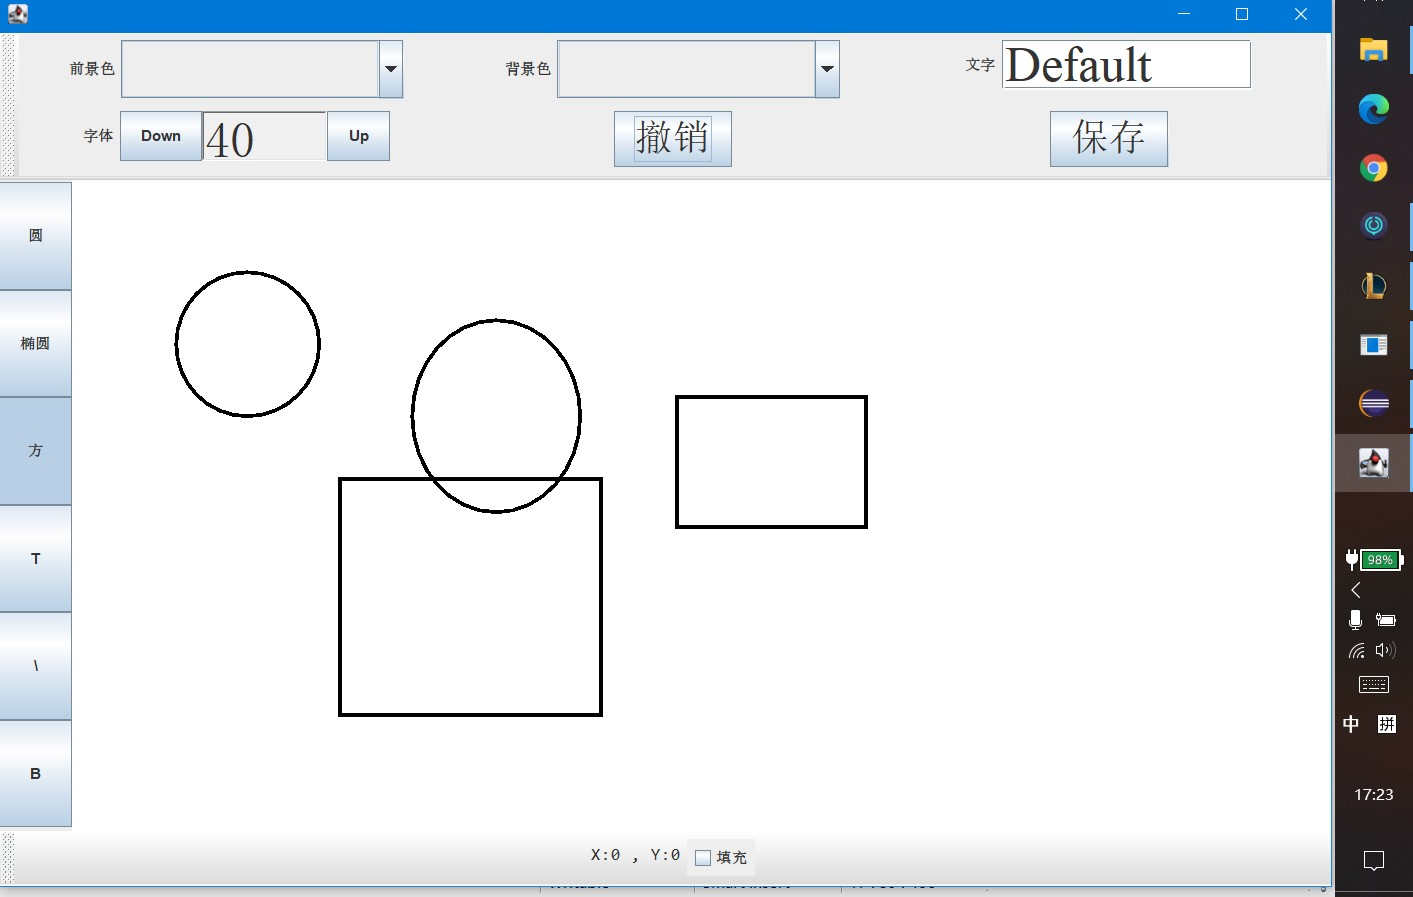
\includegraphics[scale = 0.4]{9.jpg}
    \label{fig:9}
\end{figure}
\begin{figure}[htbp]
    \centering
    \caption{另存为jpg}
    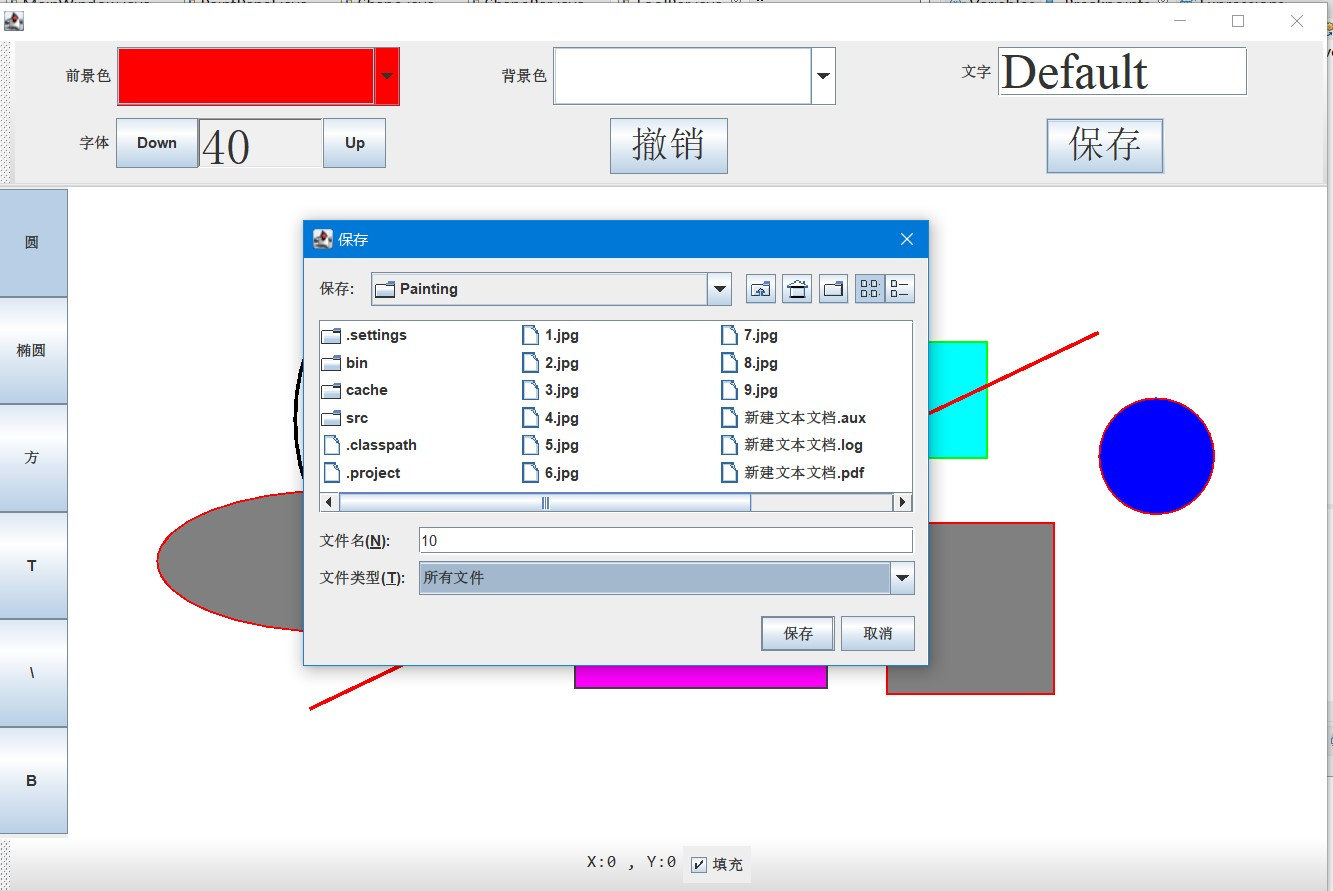
\includegraphics[scale = 0.4]{11.jpg}
    \label{fig:10}
\end{figure}
\begin{figure}[htbp]
    \centering
    \caption{存储结果}
    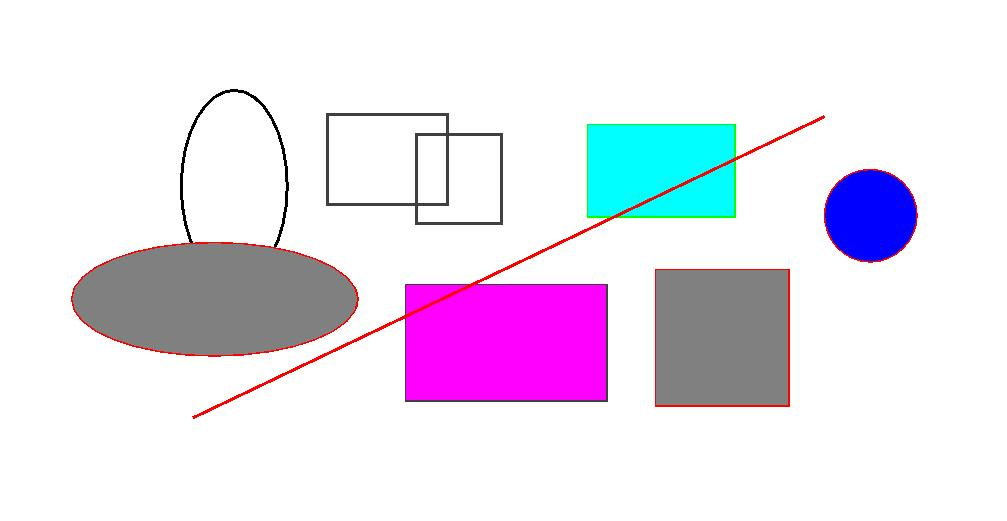
\includegraphics[scale = 0.35]{10.jpg}
    \label{fig:11}
\end{figure}
\newpage
\section{代码}
\begin{figure}[htbp]
    \centering
    \caption{组织结构}
    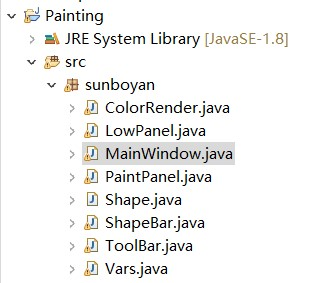
\includegraphics[scale = 0.8]{12.jpg}
    \label{fig:11}
\end{figure}
代码位于:
\begin{lstlisting}[caption = Vars.Java]
    package sunboyan;

    import ...
    public class Vars {
    
        private static ToolBar toolBar = null;
        private static JComboBox<Color> shapeColorBox = null;
        private static JComboBox<Color> backColorBox = null;
        private static JTextField textField = null;
        private static JButton upButton = null;
        private static JButton downButton = null;
        private static JPanel fontPanel = null;
        private static Color[] colors = {Color.BLACK,Color.blue,Color.CYAN,Color.DARK_GRAY, Color.GRAY,Color.GREEN,Color.LIGHT_GRAY,Color.MAGENTA,Color.ORANGE,Color.RED,Color.WHITE,Color.YELLOW};
        private static ColorRender render = null;
        private static TextField fontLabel = null;
        
        private static ShapeBar shapePanel = null;
        private static JToggleButton circleButton = null;
        private static JToggleButton squareButton = null;
        private static JToggleButton textButton = null;
        private static JToggleButton ellipseButton = null;
        private static JToggleButton lineButton = null;
        private static JToggleButton boldButton = null;
        
        private static PaintPanel paintPanel = null;
        private static Color color = Color.BLACK;
        private static Color backColor = Color.white;
        private static Shape shape = null;
        public static Shape [] items = null;
        public static int nums = 0;
        private static String shapeString = "line";
        private static Font font =null;
        
        private static LowPanel lowerPanel =null;
        private static JLabel stateLabel = null;
        private static JCheckBox checkBox  = null;
        public static boolean isFilled = false;
        public static boolean isBold = false;
        
        public static JButton saveButton = null;
        public static JButton undoButton = null;
        
        public static ToolBar getToolPanel() {
            if(toolBar == null) {
                toolBar = new ToolBar();
            }
            return toolBar;
        }

        public static JComboBox<Color> getShapeColorBox() {
            if(shapeColorBox == null) {
                shapeColorBox = new JComboBox<>(getColors());
                shapeColorBox.addItemListener(new ItemListener() {			
                    @Override
                    public void itemStateChanged(ItemEvent e) {
                        // TODO Auto-generated method stub
                        Vars.color = (Color)shapeColorBox.getSelectedItem();
                        shapeColorBox.setBackground(color);
                        shapeColorBox.setFocusable(false);
                    }
                });
                shapeColorBox.setRenderer(getColorRender());
            }
            return shapeColorBox;
        }

        public static JComboBox<Color> getBackColorBox() {
            if(backColorBox == null) {
                backColorBox = new JComboBox<>(getColors());
                backColorBox.addItemListener(new ItemListener() {
                    
                    @Override
                    public void itemStateChanged(ItemEvent e) {
                        // TODO Auto-generated method stub
                        Vars.backColor = (Color)backColorBox.getSelectedItem();
                        backColorBox.setBackground(backColor);
                        backColorBox.setFocusable(false);
                    }
                });
                backColorBox.setRenderer(getColorRender());
            }
            return backColorBox;
        }

        public static ColorRender getColorRender() {
            if(render == null) {
                render = new ColorRender();
                render.setPreferredSize(new Dimension(200,40));
            }
            return render;
        } 

        public static JTextField getTextField() {
            if(textField == null) {
                textField= new JTextField();
                textField.setPreferredSize(new Dimension(200,40));
                textField.setText("Default");
                textField.setFont(new Font("Times New Roman",Font.PLAIN,40));
            }
            return textField;
        }

        public static JButton getUpButton() {
            if(upButton == null) {
                upButton= new JButton();
                upButton.setText("Up");
                upButton.addMouseListener(new MouseAdapter() {
                    @Override
                    public void mouseReleased(MouseEvent e) {
                        addSize();
                        Integer integer = getFont().getSize();
                        getFontLabel().setText(integer.toString());
                    }
                });
            }
            return upButton;
        }

        public static JButton getDownButton() {
            if(downButton == null) {
                downButton= new JButton();
                downButton.setText("Down");
                downButton.addMouseListener(new MouseAdapter() {
                    @Override
                    public void mouseReleased(MouseEvent e) {
                        subSize();
                        Integer integer = getFont().getSize();
                        getFontLabel().setText(integer.toString());
                    }
                });
            }
            return downButton;
        }

        public static JPanel getFontPanel() {
            if(fontPanel == null) {
                fontPanel = new JPanel();
                fontPanel.setLayout(new BorderLayout());
                fontPanel.add(getFontLabel(),BorderLayout.CENTER);
                fontPanel.add(getUpButton(),BorderLayout.EAST);
                fontPanel.add(getDownButton(),BorderLayout.WEST);
            }
            return fontPanel;
        }

        public static Color [] getColors() {
            return colors;
        }

        public static TextField getFontLabel() {
            if(fontLabel == null) {
                fontLabel = new TextField();
                fontLabel.setPreferredSize(new Dimension(100,40));
                fontLabel.setEditable(false);
                fontLabel.setFont(new Font("Consolas", Font.PLAIN, 40));
                fontLabel.setText("40");
            }
            return fontLabel;
        }
    
        public static ShapeBar getShapePanel() {
            if(shapePanel == null) {
                shapePanel = new ShapeBar();
            }
            return shapePanel;
        }

        public static JToggleButton getCircleButton() {
            if(circleButton == null) {
                circleButton= new JToggleButton("圆",false);
                circleButton.setSize(60, 60);
                circleButton.addMouseListener(new MouseAdapter() {			
                    @Override
                    public void mousePressed(MouseEvent e) {
                        // TODO Auto-generated method stub
                            getSquareButton().setSelected(false);
                            getEllipseButton().setSelected(false);
                            getTextButton().setSelected(false);
                            getLineButton().setSelected(false);
                            Vars.setString("circle");
                        }
    
                });
            }
            return circleButton;
        }

        public static JToggleButton getSquareButton() {
            if(squareButton == null) {
                squareButton= new JToggleButton("方",false);
                squareButton.setSize(60,60);
                squareButton.setText("方");
                squareButton.addMouseListener(new MouseAdapter() {			
                    @Override
                    public void mousePressed(MouseEvent e) {
                        // TODO Auto-generated method stub					
                            getCircleButton().setSelected(false);
                            getEllipseButton().setSelected(false);
                            getTextButton().setSelected(false);	
                            getLineButton().setSelected(false);
                            Vars.setString("square");
                    }
    
                });
            }
            return squareButton;
        }

        public static JToggleButton getEllipseButton() {
            if(ellipseButton == null) {
                ellipseButton= new JToggleButton("椭圆",false);
                ellipseButton.setSize(60,60);
                ellipseButton.addMouseListener(new MouseAdapter() {			
                    @Override
                    public void mousePressed(MouseEvent e) {
                        // TODO Auto-generated method stub
                            getCircleButton().setSelected(false);
                            getSquareButton().setSelected(false);
                            getTextButton().setSelected(false);
                            getLineButton().setSelected(false);
                            Vars.setString("ellipse");
                    }
    
                });
            }
            return ellipseButton;
        }

        public static JToggleButton getTextButton() {
            if(textButton == null) {
                textButton= new JToggleButton("T",false);
                textButton.setSize(60,60);
                textButton.addMouseListener(new MouseAdapter() {			
                    @Override
                    public void mousePressed(MouseEvent e) {
                        // TODO Auto-generated method stub
                            getCircleButton().setSelected(false);
                            getSquareButton().setSelected(false);
                            getEllipseButton().setSelected(false);
                            getLineButton().setSelected(false);
                            Vars.setString("text");
                    }
    
                });
            }
            return textButton;
        }

        public static JToggleButton getLineButton() {
            if(lineButton == null) {
                lineButton = new JToggleButton("\\",false);
                lineButton.setSize(60,60);
                lineButton.addMouseListener(new MouseAdapter() {			
                    @Override
                    public void mousePressed(MouseEvent e) {
                        // TODO Auto-generated method stub
                            getCircleButton().setSelected(false);
                            getSquareButton().setSelected(false);
                            getEllipseButton().setSelected(false);
                            getTextButton().setSelected(false);
                            Vars.setString("line");
                    }
    
                });
            }
            return lineButton;
        }

        public static JToggleButton getBoldButton() {
            if(boldButton==null) {
                boldButton = new JToggleButton("B");
                boldButton.addItemListener(new ItemListener() {
                    
                    @Override
                    public void itemStateChanged(ItemEvent e) {
                        // TODO Auto-generated method stub
                        isBold = boldButton.isSelected();
                        System.out.println(isBold);
                    }
                });
            }
            return boldButton;
        }

        public static JButton getUndoButton() {
            if(undoButton == null) {
                undoButton = new JButton("撤销");
                undoButton.setFont(new Font("宋体",Font.PLAIN,30));
                undoButton.addMouseListener(new MouseAdapter() {
                    @Override
                    public void mouseReleased(MouseEvent e) {
                        subItems();
                        paintPanel.repaint();
                    }
                });
            }
            return undoButton;
            
        }

        public static JButton getSaveButton() {
            if(saveButton == null) {
                saveButton = new JButton("保存");
                saveButton.setFont(new Font("宋体",Font.PLAIN,30));
                saveButton.addMouseListener(new MouseAdapter() {
                    @Override
                    public void mouseReleased(MouseEvent e) {
                        getPaintPanel().save();
                    }
                });
            }
            return saveButton;
        }

        public static Color getColor() {
            return color;
        }

        public static void setColor(Color c) {
            color = c;
        }

        public static Color getBackColor() {
            return backColor;
        }

        public static void setBackColor(Color c) {
            backColor = c;
        }

        public static Shape getShape() {
            if(shape == null) {
                shape = new Shape();
            }
            return shape;
        }

        public static Shape[] getItems() {
            if(items ==null) {
                items = new Shape[100];
            }
            return items;
        }

        public static int getNums() {
            return nums;
        }

        public static void addItems() {
            items[nums] = new Shape(shape);
            nums++;
        }

        public static void subItems() {
            if(nums>0) {
                items[--nums] = null;
            }
        }

        public static void setString(String string) {
            shapeString = string;
        }

        public static String getString() {
            return shapeString;
        }

        public static PaintPanel getPaintPanel() {
            if(paintPanel == null) {
                paintPanel = new PaintPanel();
            }
            return paintPanel;
        }

        public static Font getFont() {
            if(font==null) {
                font = new Font("Times New Roman", Font.PLAIN, 40);
            }
            return font;
        }

        public static void addSize() {
            if(font==null) {
                font = new Font("Times New Roman", Font.PLAIN, 42);
            }else if(font.getSize()<80){
                font = new Font("Times New Roman",Font.PLAIN,font.getSize()+2);
            }	
        }

        public static void subSize() {
            if(font==null) {
                font = new Font("Times New Roman", Font.PLAIN, 38);
            }else if(font.getSize()>2) {
                font = new Font("Times New Roman",Font.PLAIN,font.getSize()-2);
            }	
        }

        public static  LowPanel getLowPanel() {
            if(lowerPanel ==null) {
                lowerPanel = new LowPanel();
            }
            return lowerPanel;
        }

        public static JLabel getStateLabel() {
            if(stateLabel ==null) {
                stateLabel = new JLabel();
                stateLabel.setFont(new Font("Consolas", Font.PLAIN, 14));
                stateLabel.setText("X:0 , Y:0");
            }
            return stateLabel;
        }

        public static JCheckBox getCheckBox() {
            if (checkBox == null) {
                checkBox = new JCheckBox("填充");
                checkBox.addItemListener(new ItemListener() {
                    
                    @Override
                    public void itemStateChanged(ItemEvent e) {
                        // TODO Auto-generated method stub
                        isFilled = checkBox.isSelected();
                    }
                } );
            }
            return checkBox;
        }
    }       
\end{lstlisting}

\begin{lstlisting}[caption = PaintPanel.java]
    package sunboyan;
    import ...
    public class PaintPanel extends JPanel implements MouseListener,MouseMotionListener{
        private static final long serialVersionUID = 1L;
    
        @Override
        public void mouseClicked(MouseEvent e) {
            // TODO Auto-generated method stub
            
        }
    
        @Override
        public void mousePressed(MouseEvent e) {
            // TODO Auto-generated method stub
            int x1 = e.getX();
            int y1 = e.getY();
            Vars.getShape().setX1(x1);
            Vars.getShape().setY1(y1);
        }
    
        @Override
        public void mouseReleased(MouseEvent e) {
            // TODO Auto-generated method stub
            int x2 = e.getX();
            int y2 = e.getY();
            Vars.getShape().setX2(x2);
            Vars.getShape().setY2(y2);
            Vars.getShape().setColor();
            Vars.getShape().setString();
            Vars.getShape().setFont(Vars.getFont());
            Vars.getShape().setBackColor(Vars.getBackColor());
            Vars.getShape().setTextString(Vars.getTextField().getText());
            Vars.getShape().filled = Vars.isFilled;
            Vars.getShape().bold = Vars.isBold;
            Vars.addItems();
            paintComponent(getGraphics());
        }
        
        @Override
        public void mouseExited(MouseEvent e) {
            // TODO Auto-generated method stub
            Vars.getStateLabel().setText("X:0 , Y:0");
        }
        
        
    
        @Override
        public void mouseDragged(MouseEvent e) {
            // TODO Auto-generated method stub
            
        }
    
        @Override
        public void mouseMoved(MouseEvent e) {
            // TODO Auto-generated method stub
            Vars.getStateLabel().setText("X:"+e.getX()+" , Y:"+e.getY());
        }
    
        public PaintPanel() {
            setBackground(Color.white);
            setCursor(Cursor.getPredefinedCursor(Cursor.CROSSHAIR_CURSOR));
            addMouseListener(this);
            addMouseMotionListener(this);
        }
        
        @Override
        public void paintComponent(Graphics g) {
            super.paintComponent(g);
            try {
                g.drawImage(ImageIO.read(new File("D:\\Coding projects\\eclipse-workspace\\Painting\\cache\\autosave.jpg")), 0, 0, Color.WHITE, this);
            } catch (IOException e) {
                // TODO Auto-generated catch block
                ;
            }
            setBackground(Vars.getBackColor());
            Shape[] shapes = Vars.getItems();
            if(shapes == null) {
                return;
            }
            for (Shape shape : shapes) {
                draw((Graphics2D)g, shape);
            }
            if(Vars.nums>10) {
                clear();
            }
        }
        public void clear() {
            Vars.nums = 0;
            autoSave();
            Vars.items = new Shape[100];	
        }
        
        public void draw(Graphics2D g, Shape shape) {
            if(shape ==null) {
                return;
            }
            switch (shape.getString()) {
            case "circle":
                g.setColor(shape.getColor());
                if(shape.bold) {
                    g.setStroke(new BasicStroke(10));
                }else {
                    g.setStroke(new BasicStroke(3));
                }
                g.drawOval(Math.min(shape.getX1(), shape.getX2()), Math.min(shape.getY1(), shape.getY2()), Math.abs(shape.getX1()-shape.getX2()), Math.abs(shape.getX1()-shape.getX2()));
                if (shape.filled) {
                    g.setColor(shape.getBackColor());
                    g.fillOval(Math.min(shape.getX1(), shape.getX2()), Math.min(shape.getY1(), shape.getY2()), Math.abs(shape.getX1()-shape.getX2()), Math.abs(shape.getX1()-shape.getX2()));
    
                }else {
    
                }
                break;
            case "square":
                g.setColor(shape.getColor());
                if(shape.bold) {
                    g.setStroke(new BasicStroke(10));
                }else {
                    g.setStroke(new BasicStroke(3));
                }
                g.drawRect(Math.min(shape.getX1(), shape.getX2()), Math.min(shape.getY1(), shape.getY2()), Math.abs(shape.getX1()-shape.getX2()), Math.abs(shape.getY1()-shape.getY2()));
                if (shape.filled) {
                    g.setColor(shape.getBackColor());
                    g.fillRect(Math.min(shape.getX1(), shape.getX2()), Math.min(shape.getY1(), shape.getY2()), Math.abs(shape.getX1()-shape.getX2()), Math.abs(shape.getY1()-shape.getY2()));
    
                }else {
    
                }
                break;
            case "ellipse":
                g.setColor(shape.getColor());
                if(shape.bold) {
                    g.setStroke(new BasicStroke(10));
                }else {
                    g.setStroke(new BasicStroke(3));
                }
                g.drawOval(Math.min(shape.getX1(), shape.getX2()), Math.min(shape.getY1(), shape.getY2()), Math.abs(shape.getX1()-shape.getX2()), Math.abs(shape.getY1()-shape.getY2()));
                if (shape.filled) {
                    g.setColor(shape.getBackColor());
                    g.fillOval(Math.min(shape.getX1(), shape.getX2()), Math.min(shape.getY1(), shape.getY2()), Math.abs(shape.getX1()-shape.getX2()), Math.abs(shape.getY1()-shape.getY2()));
    
                }else {
                }
                break;			
            case "text":
                g.setColor(shape.getColor());
                if(shape.bold) {
                    Font font = shape.getFont().deriveFont(Font.BOLD);
                    g.setFont(font);
                }else {
                    g.setFont(shape.getFont());
                }
                g.drawString(shape.getTextString(),Math.min(shape.getX1(), shape.getX2()), Math.min(shape.getY1(), shape.getY2()));
                break;
            case "line":
                g.setColor(shape.getColor());
                if(shape.bold) {
                    g.setStroke(new BasicStroke(10));
                }else {
                    g.setStroke(new BasicStroke(3));
                }
                g.drawLine(shape.getX1(), shape.getY1(), shape.getX2(), shape.getY2());
                break;
            default:
                break;
            }
        }
    
        @Override
        public void mouseEntered(MouseEvent e) {
            // TODO Auto-generated method stub
            
        }
    
        public void save() {
            BufferedImage image  = new BufferedImage(getWidth(), getHeight(), BufferedImage.TYPE_INT_RGB);
            Graphics2D g = (Graphics2D)image.getGraphics();
            paint(g);
            JFileChooser chooser=new JFileChooser();//文件保存对话框
            chooser.setCurrentDirectory(new File("."));
            if(chooser.showSaveDialog(null)==JFileChooser.APPROVE_OPTION){
                File oFile=chooser.getSelectedFile();
                try{
                     File file = new File(oFile.getName()+".jpg");
                    ImageIO.write(image, "jpg", file);//保存图像文件
                }catch(IOException ex){
                    ex.printStackTrace();
                }
            }
        }
        public void autoSave() {
            BufferedImage image  = new BufferedImage(getWidth(), getHeight(), BufferedImage.TYPE_INT_RGB);
            Graphics2D g = (Graphics2D)image.getGraphics();
            paint(g);
            try {
                File cacheFile = new File("D:\\Coding projects\\eclipse-workspace\\Painting\\cache\\autosave.jpg");
                ImageIO.write(image, "jpg", cacheFile);
            } catch (Exception e) {
                // TODO: handle exception
            }
        }
    }      
\end{lstlisting}
\begin{lstlisting}[caption = ToolBar.java]
    package sunboyan;

    import ...
    public class ToolBar extends JToolBar{
        private JPanel panel1 = null;
        private JPanel panel2 = null;
        private JPanel panel3 = null;
        private JPanel panel4 = null;
        private JPanel panel5 = null;
        private JPanel panel6 = null;
        public ToolBar() {
            panel1 = new JPanel();
            panel2 = new JPanel();
            panel3 = new JPanel();
            panel4 = new JPanel();
            panel5 = new JPanel();
            panel6 = new JPanel();
            panel2.add(new JLabel("背景色"));
            panel2.add(Vars.getBackColorBox());
            panel1.add(new JLabel("前景色"));
            panel1.add(Vars.getShapeColorBox());
            panel3.add(new JLabel("文字"));
            panel3.add(Vars.getTextField());
            panel4.add(new JLabel("字体"));
            panel4.add(Vars.getFontPanel());
            panel5.add(Vars.getUndoButton());
            panel6.add(Vars.getSaveButton());
            setLayout(new GridLayout(2,3));
            add(panel1,getLayout());
            add(panel2,getLayout());
            add(panel3,getLayout());
            add(panel4,getLayout());
            add(panel5,getLayout());
            add(panel6,getLayout());
        }
        
    }     
\end{lstlisting}
\begin{lstlisting}[caption = shape.java]
    package sunboyan;

    import java.awt.Color;
    import java.awt.Font;
    
    public class Shape {
        private int x1 = 0;
        private int x2 = 0;
        private int y1 = 0;
        private int y2 = 0;
        private String string = null;
        private String textString =null;
        private Color color = null;
        private Color backColor = null;
        private Font font = new Font("Times New Roman",Font.PLAIN,20);
        public boolean filled =false;
        public boolean bold = false;
        public int getX1() {
            return x1;
        }
        public void setX1(int x1) {
            this.x1 = x1;
        }
        public int getX2() {
            return x2;
        }
        public void setX2(int x2) {
            this.x2 = x2;
        }
        public int getY1() {
            return y1;
        }
        public void setY1(int y1) {
            this.y1 = y1;
        }
        public int getY2() {
            return y2;
        }
        public void setY2(int y2) {
            this.y2 = y2;
        }
        public String getString() {
            return string;
        }
        public void setString() {
            this.string = Vars.getString();
        }
        public Color getColor() {
            return color;
        }
        public void setColor() {
            color = Vars.getColor();
        }
        public void setFont(Font font) {
            this.font = font;
        }	
        public Font getFont() {
            return font;
        }
        public Color getBackColor() {
            return backColor;
        }
        public void setBackColor(Color c) {
            backColor =c;
        }
        public Shape() {
            
        }
        public Shape(Shape shape) {
            string = shape.string;
            color = shape.color;  
            backColor = shape.backColor;
            font = shape.font;
            filled =shape.filled;
            bold = shape.bold;
            textString = shape.textString;
            x1 = shape.x1;
            x2 = shape.x2;
            y1 = shape.y1;
            y2 = shape.y2;
        }
        public String getTextString() {
            return textString;
        }
        public void setTextString(String string) {
            textString = string;
        }
    }        
\end{lstlisting}
\begin{lstlisting}[caption = shapeBar.java]
    package sunboyan;

    import java.awt.FlowLayout;
    import java.awt.GridBagLayout;
    import java.awt.GridLayout;
    import javax.swing.JPanel;
    import javax.swing.JToggleButton;
    
    public class ShapeBar extends JPanel {
        private static JToggleButton circleButton = null;
        private static JToggleButton squareButton = null;
        private static JToggleButton textButton = null;
        private static JToggleButton ellipseButton = null;
        private static JToggleButton lineButton = null;
        private static JToggleButton boldButton = null;
        public ShapeBar() {
            circleButton = Vars.getCircleButton();
            squareButton = Vars.getSquareButton();
            textButton = Vars.getTextButton();
            ellipseButton = Vars.getEllipseButton();
            lineButton = Vars.getLineButton();
            boldButton = Vars.getBoldButton();
            setLayout(new GridLayout(6,1));
            add(circleButton);
            add(ellipseButton);
            add(squareButton);
            add(textButton);
            add(lineButton);
            add(boldButton);
        }      
}        
\end{lstlisting}
\begin{lstlisting}[caption = LowPanel.java]
    package sunboyan;

    import java.awt.FlowLayout;
    import javax.swing.JCheckBox;
    import javax.swing.JLabel;
    import javax.swing.JPanel;
    import javax.swing.JToolBar;
    
    public class LowPanel extends JToolBar{
        private static JLabel stateLabel = null;
        private static JCheckBox checkBox =null;
        public LowPanel() {
            stateLabel = Vars.getStateLabel();
            checkBox = Vars.getCheckBox();
            setLayout(new FlowLayout(FlowLayout.CENTER));
            add(stateLabel);
            add(checkBox);
        }
    }      
\end{lstlisting}
\begin{lstlisting}[caption = ColorRender.java]
    package sunboyan;

    import ...
    public class ColorRender extends JLabel implements ListCellRenderer<Color>{
    
        private static final long serialVersionUID = 1L;
        public ColorRender() {
            setOpaque(true);
            setHorizontalAlignment(CENTER);
            setVerticalAlignment(CENTER);
        }
        @Override
        public Component getListCellRendererComponent(JList list, Color value, int index, boolean isSelected,
                boolean cellHasFocus) {
            // TODO Auto-generated method stub
            if(index == -1) {
                
            }else {
                setBackground(value);
            }
            return this;
        } 
        
    }    
\end{lstlisting}
\begin{lstlisting}[caption = MainWindow.java]
    package sunboyan;

    import ...
    public class MainWindow extends JFrame{
        public static void main(String[]args) {
            EventQueue.invokeLater(new Runnable() {
                public void run() {
                    try {
                        MainWindow frame = new MainWindow();
                        frame.setVisible(true);
                    } catch (Exception e) {
                        e.printStackTrace();
                    }
                }
            });
        }
        public MainWindow() {
            JPanel panel = new JPanel();
            setContentPane(panel);
            setDefaultCloseOperation(EXIT_ON_CLOSE);
            setBounds(0, 0, 1080, 720);
            getContentPane().setLayout(new BorderLayout());
            getContentPane().add(Vars.getToolPanel(), BorderLayout.NORTH);
            getContentPane().add(Vars.getShapePanel(),BorderLayout.WEST);
            getContentPane().add(Vars.getPaintPanel(),BorderLayout.CENTER);
            getContentPane().add(Vars.getLowPanel(),BorderLayout.SOUTH);
        }
        public void update(Graphics g) {
            // TODO Auto-generated method stub
            super.update(g);
            Vars.getPaintPanel().paintComponent(g);
        }
    }        
\end{lstlisting}
\end{document}